
\documentclass[11pt, a4paper]{article}
\usepackage[top=1in,bottom=1in,left=0.5in,right=0.5in]{geometry}
\usepackage{graphicx}
\usepackage{amsmath}
\usepackage{natbib}
\usepackage{url}
\newcommand{\BibTeX}{{\sc Bib}\TeX}
\begin{document}


\title{Rube Goldberg Simulation : CS296 Group 25 Project Report.}
\author{Anmol Garg\\
110050020\\
\texttt{anmolgarg@cse.iitb.ac.in}\\
\and
Anshul Purohit\\
110050002\\
\texttt{anshulp@cse.iitb.ac.in}}
\date{\today}
\maketitle

\fontsize{11pt}{15pt}\selectfont

\section{Introduction}
This report presents our original design and finished design for the Rube Goldberg Machine \cite{RG} and describes its features.It begins by stating the deviations from our original and finished design. We have analysed our code for the simulation through the timing and profiling experiments. \\
Then it also compares the profiles generated by gprof for two different compiling modes. Gprof \cite{GProf} is a inbuilt profiler in Linux. A profiler identifies the portion of code that takes large time which can be then optimized. The profiler also generates a call graph showing the callee-caller relationship which is breifly explained at the end.

\section{Original Design}

This section describes about the design, features and elements of the Rube Goldberg Machine which we initially made three months ago. However, in implementing this with Box2D \cite{Box2D} API we had to modify our design slightly and add other intresting features which will be described shortly. \\

Following is our original design and its description. \\

\begin{center}
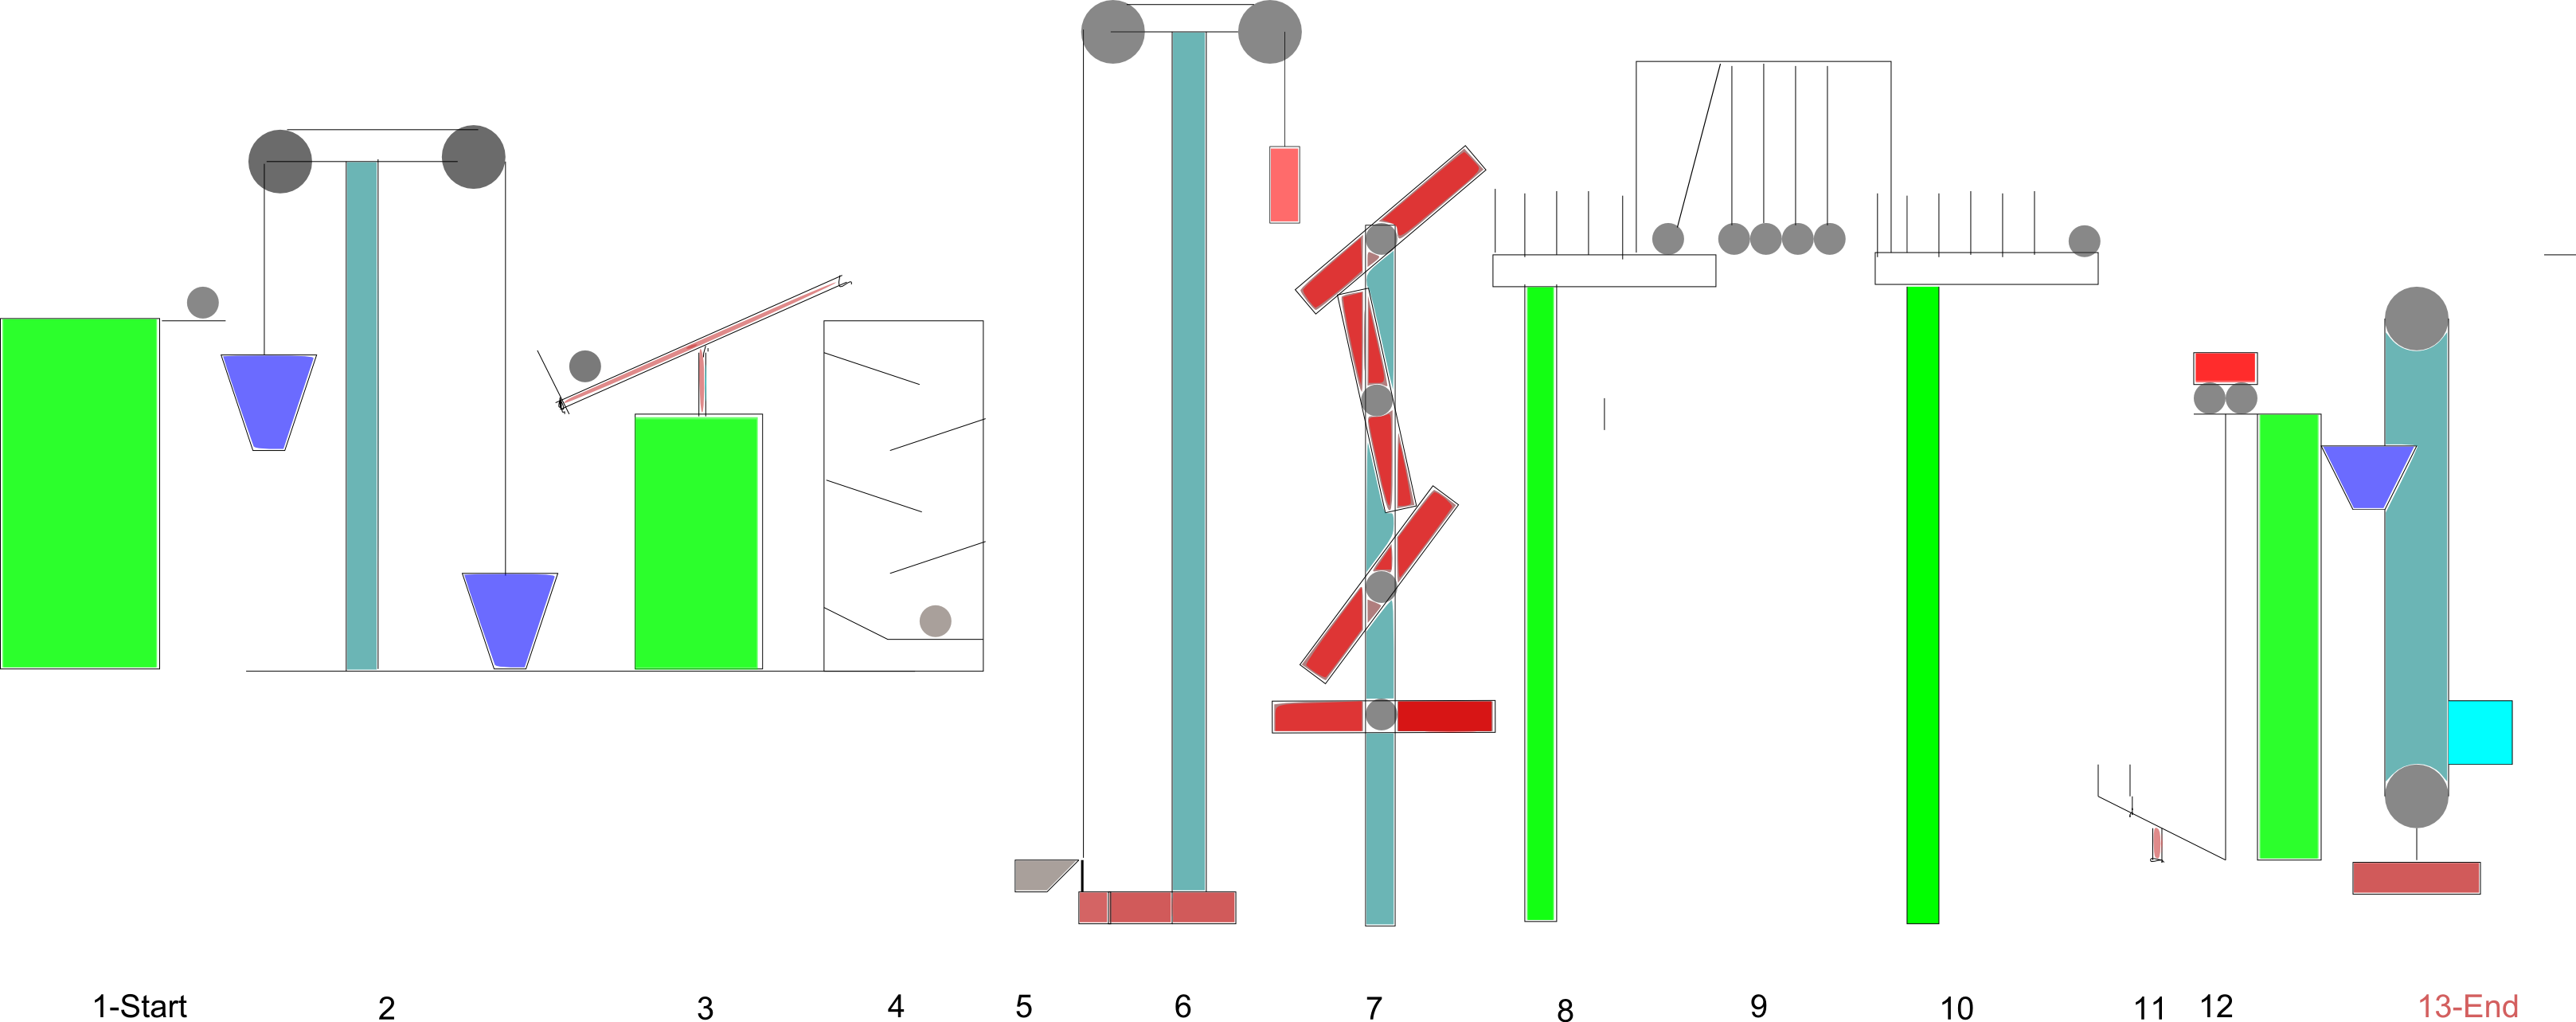
\includegraphics[width = 16cm]{ReportImages/RubeGoldbergDesign.eps}
\end{center} 

\begin{itemize}
\item Windup robot toy is released. Toy moves rightward across platform, knocking the ball off the platform.
\item The ball rolls off of the platform and falls into cup A. This upsets the balance of the Atwood Machine,
causing cup A to accelerate downward while cup B accelerates upward.
\item Cup B knocks the left side of the lever upwards. The lifting up of the left side of the lever causes a steel
marble to roll downwards into the set of marble tracks.
\item The marble zigzags down the angled tracks. During the first section, the marble rolls through a set of
chimes of varying length. After the last ramp, the steel marble collides with a lighter steel ball.
\item The ball rolls from the angled tracks into a funnel where it falls onto the trigger of a mousetrap.
\item The mousetrap goes off, with its metal arm swinging from left to right.
\item The clothespin is squeezed open by the swinging arm of the mousetrap, releasing a string.
\item The released string causes the weight on the opposite side of the pulley system to accelerate downwards.
\item The downward accelerating mass collides with the arm of a rotating lever. The bottom lever spins
counter-clockwise, knocking into the arm of the lever above it. The levers continue to spin, transferring
the energy upward to the top lever.
\item The top lever swings into a domino, beginning another chain of falling dominoes. The final domino
collides with a ball from a Newton’s Cradle \cite{RHK} toy that sits perched on the platform with the dominoes.
\item The first ball of the Newton’s Cradle swings into the other four balls. The rightmost ball swings
forward, knocking into a domino on the adjacent platform where they initiate another chain of domino
collisions, eventually knocking into a marble.
\item The marble rolls down through the curved tubing into the left compartment of a lever.
\item The weight of the marble causes the left side of the lever to move. The upward motion of the right side
of the lever lifts the rod that supports the platform above.
\item The left side of the platform lifts upwards, causing the car to roll downwards from left to right,
eventually falling into a cup that is attached to a string and pulley system.
\item The car falling into the cup causes the cup to accelerate downwards. The string on the opposite side of
the pulleys moves upwards, raising the flag and completing the simulation.

\end{itemize}

\section{Design Implemented}

Following is the design we implemented using the Box2D API. 

\begin{center}
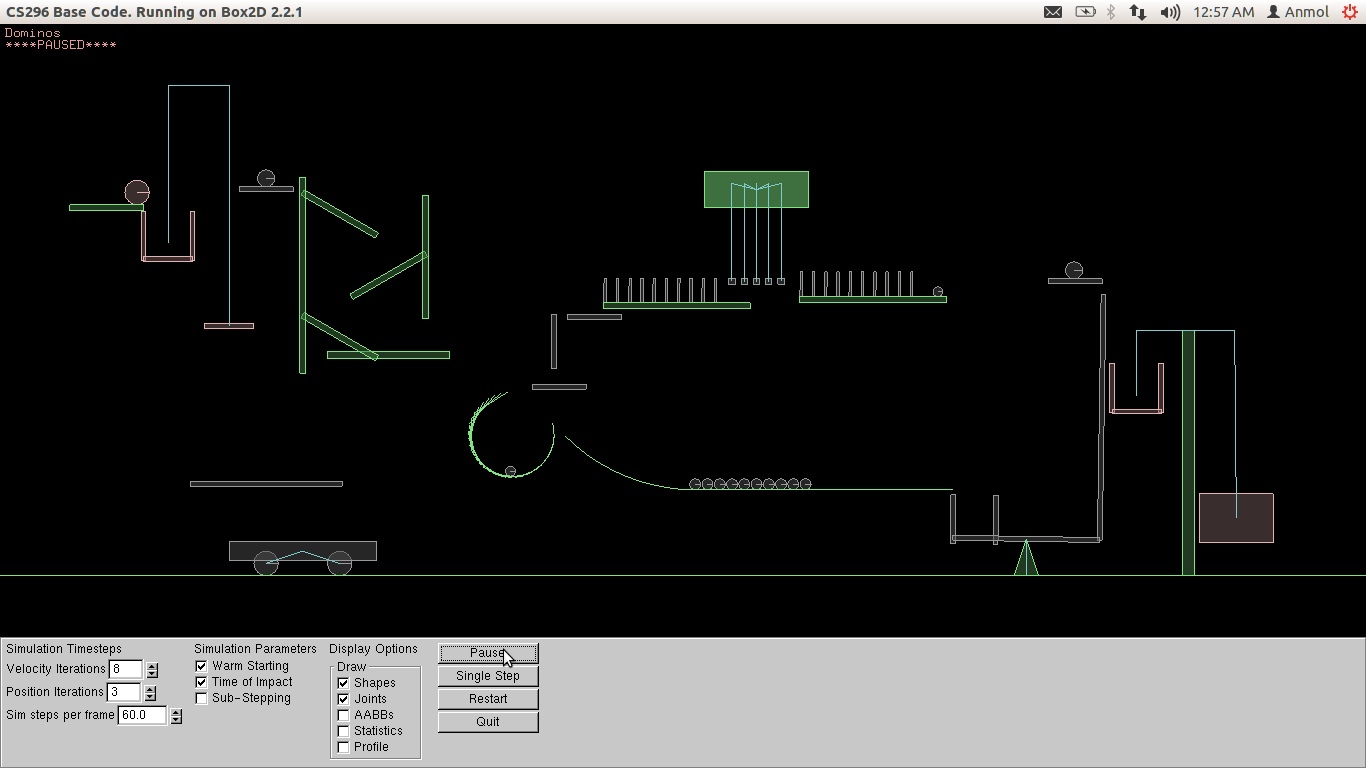
\includegraphics[width = 12cm]{ReportImages/RubeGoldbergSimulation.eps}
\end{center} 

\begin{itemize}
\item A heavy ball is released on the platform.The ball moves rightward across platform.

\begin{center}
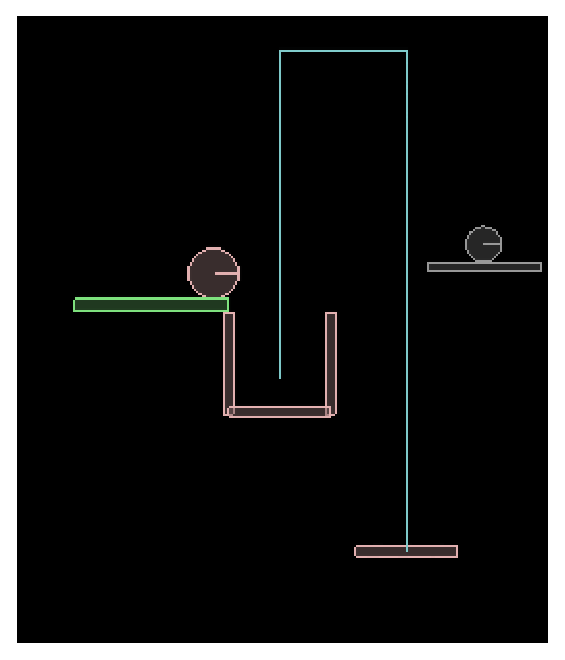
\includegraphics[width = 6cm]{ReportImages/init.eps}
\end{center} 

\item The ball rolls off of the platform and falls into cup A. This upsets the balance of the Atwood Machine,
causing cup A to accelerate downward while cup B accelerates upward.
\item Cup A knocks the big horizontal bar that triggers the motion of the car.

\begin{center}
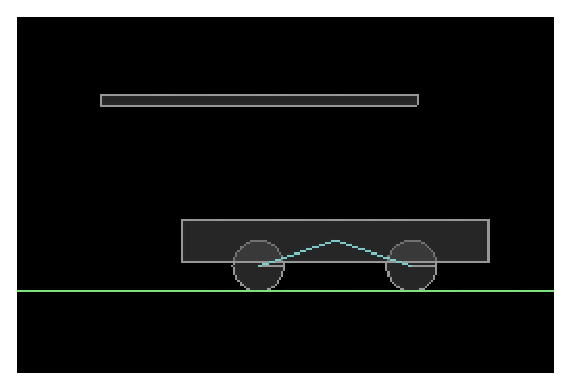
\includegraphics[width = 6cm]{ReportImages/car.eps}
\end{center} 


\item Cup B knocks the left side of the lever upwards. The lifting up of the left side of the lever causes a steel
marble to roll downwards into the set of marble tracks(ramp).
\item The marble zigzags down the angled tracks. During the first section, the marble rolls through a set of
chimes of varying length. After the last stage, the marble falls into the circular loop. Where it collides with a ligher ball.

\begin{center}
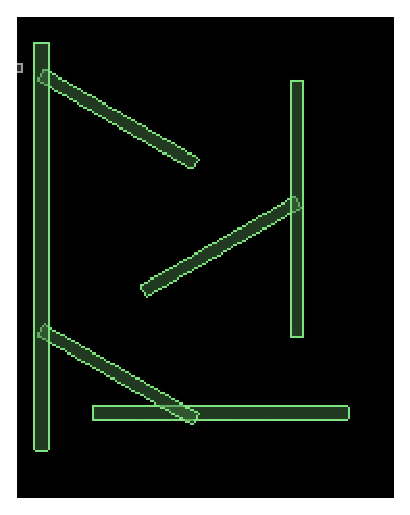
\includegraphics[width = 6cm]{ReportImages/ramp.eps}
\end{center} 


\item The lighter ball takes off and completes the vertical loop to hit a system of three rotatable bars. And the falls on a curve that conatains 10 small balls on it.

\begin{center}
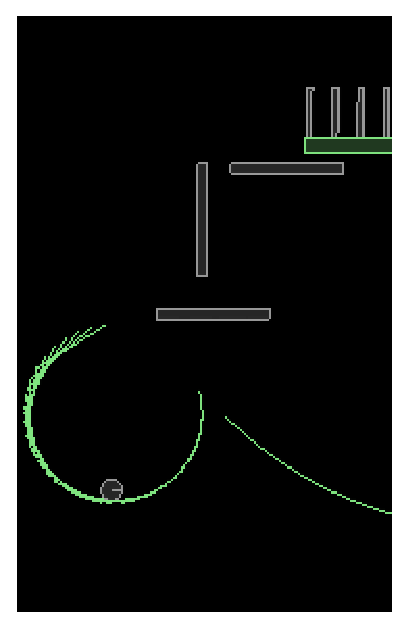
\includegraphics[width = 6cm]{ReportImages/loop.eps}
\end{center} 


\item The collision results in an angular momentum on the first horizontal bar trigerring collision with the vertical bar.
\item The vertical bar then rotates to collide with the horizontal bar.

\begin{center}
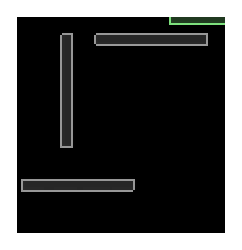
\includegraphics[width = 6cm]{ReportImages/rods.eps}
\end{center} 


\item The bar swings into a domino, beginning another chain of falling dominoes. The final domino
collides with a ball from a Newton’s Cradle toy that sits perched on the platform with the dominoes.
\item The first ball of the Newton’s Cradle swings into the other four balls. The rightmost ball swings
forward, knocking into a domino on the adjacent platform where they initiate another chain of domino
collisions, eventually knocking into a marble.

\begin{center}
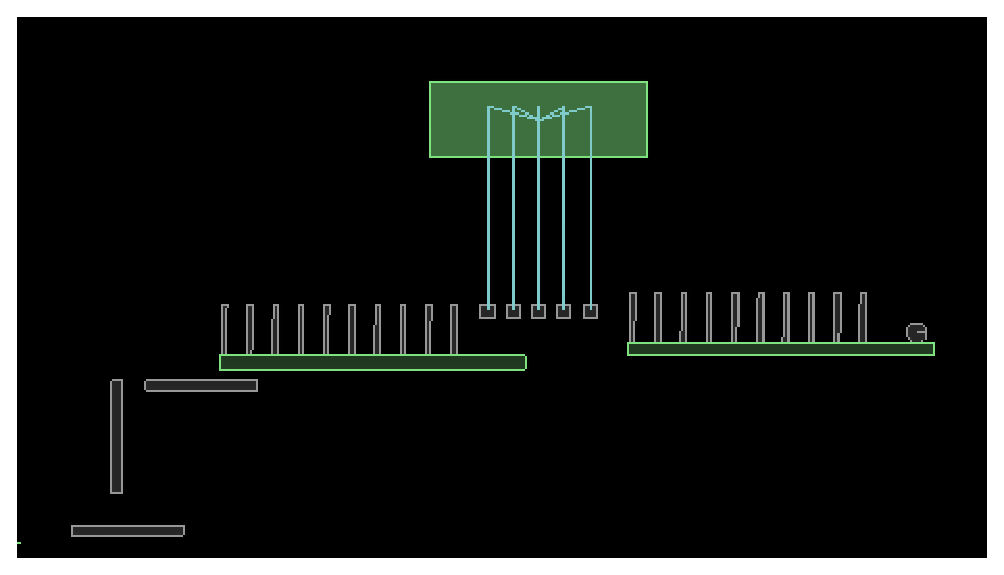
\includegraphics[width = 6cm]{ReportImages/domino.eps}
\end{center} 


\item The marble rolls falls into the left compartment of a lever. In the meanwhile, the 11 balls on the curve are also headed for the compartment of the lever and the car also reaches the lever.
\item The weight of the marbles causes the left side of the lever to move. The upward motion of the right side
of the lever lifts the rod that hits the platform above.

\begin{center}
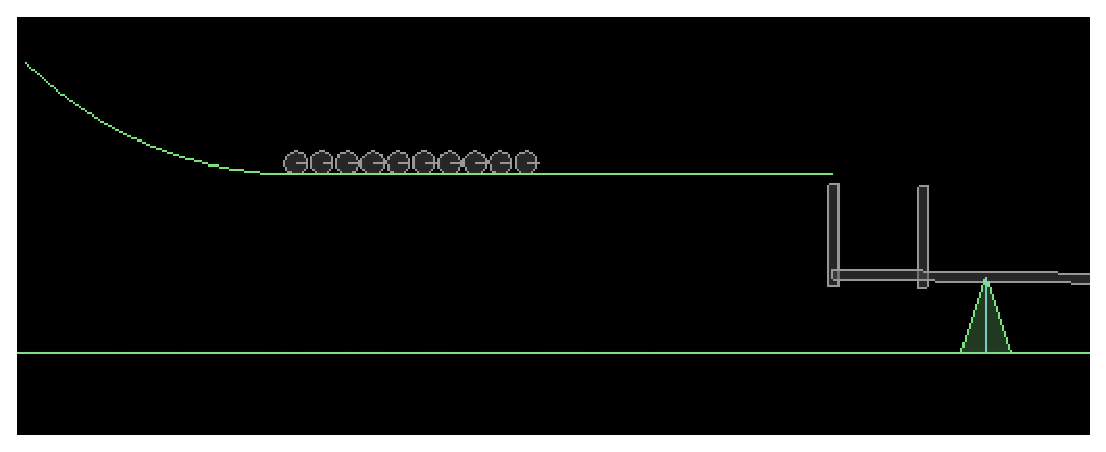
\includegraphics[width = 6cm]{ReportImages/curve.eps}
\end{center} 


\item The left side of the platform lifts upwards, causing the heavy ball to roll downwards from left to right,
eventually falling into a cup that is attached to a string and pulley system.
\item The car falling into the cup causes the cup to accelerate downwards. The string on the opposite side of
the pulleys moves upwards, raising the flag and finishing the simulation.

\begin{center}
\includegraphics[width = 6cm]{ReportImages/see-saw.eps}
\end{center} 


\end{itemize}

\section {Changes we made in the Design}

\begin{itemize}
\item We replaced the portion of simulation wherein the rope is cut to release the load with the portion where the ball takes the vertical loop. This was primarily beacuse we couldn't find a easy way to cut ropes and secondarily because the design got more interesting by replacing a pulley with anothe element.
\item We slightly modified the system of rotatable bars to include bar with initial vertical configuration. This way we could transfer more momentum to the dominos and subsequent elements.
\item We added the car and the horizontal bar that triggers its motion in our design in accordance with the theme of our simulation.Similarly, we also added curves to collect the balls into the compartment of the lever. 


\end{itemize}

\section {Interesting Features of our Design}

The name of our Design is the Flag Hoisting Rube Goldberg Machine. As is clear from the name, the interesting feature in our design is that we look forward to show the celebrations on Republic Day using our simple Design. \\
What are the interesting things you get to see on Republic Day? Here our some of them... \\
\begin{itemize}
\item All of us have undoubtly been very fond of parades on Republic Day and have definitely watched it on Television. Thus we have placed a small cart at the left end which marks the beginning of the simulation and shows the parade moving towards right as on Republic Day.
\item When Republic Day is celebrated in School we get sweets (Ladoos, It was the main reason i used to to go to school :D ). Following similar pattern we have also made a container at the right end which you can see is initially empty but as the parade moves forward and the ceremony is nearly ending we fill it with ladoos placed in the long horizontal platform. People who come to see the parade and demonstrations can collect it from the container when they leave.
\item The most prestigious part of the Republic Day ceremony - Hoisting of the Indian National Flag. This is also the motive of our Rube Goldberg Machine. Our Simulation ends with the Indian National Flag rising high and "Jan Gan Man" played in the background and all the parade standing in attention.
  
\end{itemize}
       
\section{Analysis of Plots using matplotlib \cite{plot}}

The first step of plotting involved generating data for iterations ranging from 1-100. For each iteration the script was rerun 100 times to generate sufficient data for analysis. The graphs plotted were as follows \\ 
%1) Average Step Time \& Average Loop Time Vs Iteration Values \\
%2) Average Collision Time , Velocity \& Position Updates Vs Iteration Values \\ 
%3) Average Step Time \& Average Loop Time Vs Rerun Values \\ 
%4) Average Collision Time , Velocity \& Position Updates Vs Iteration Values \\
%5) Step Time (with error-bars) Vs Iteration Values \\
%6) Step Time frequency \& cumulative frequency plot (for a fixed iteration value) \\

\subsection{Average Step Time \& Average Loop Time Vs Iteration Values}
\begin{center}
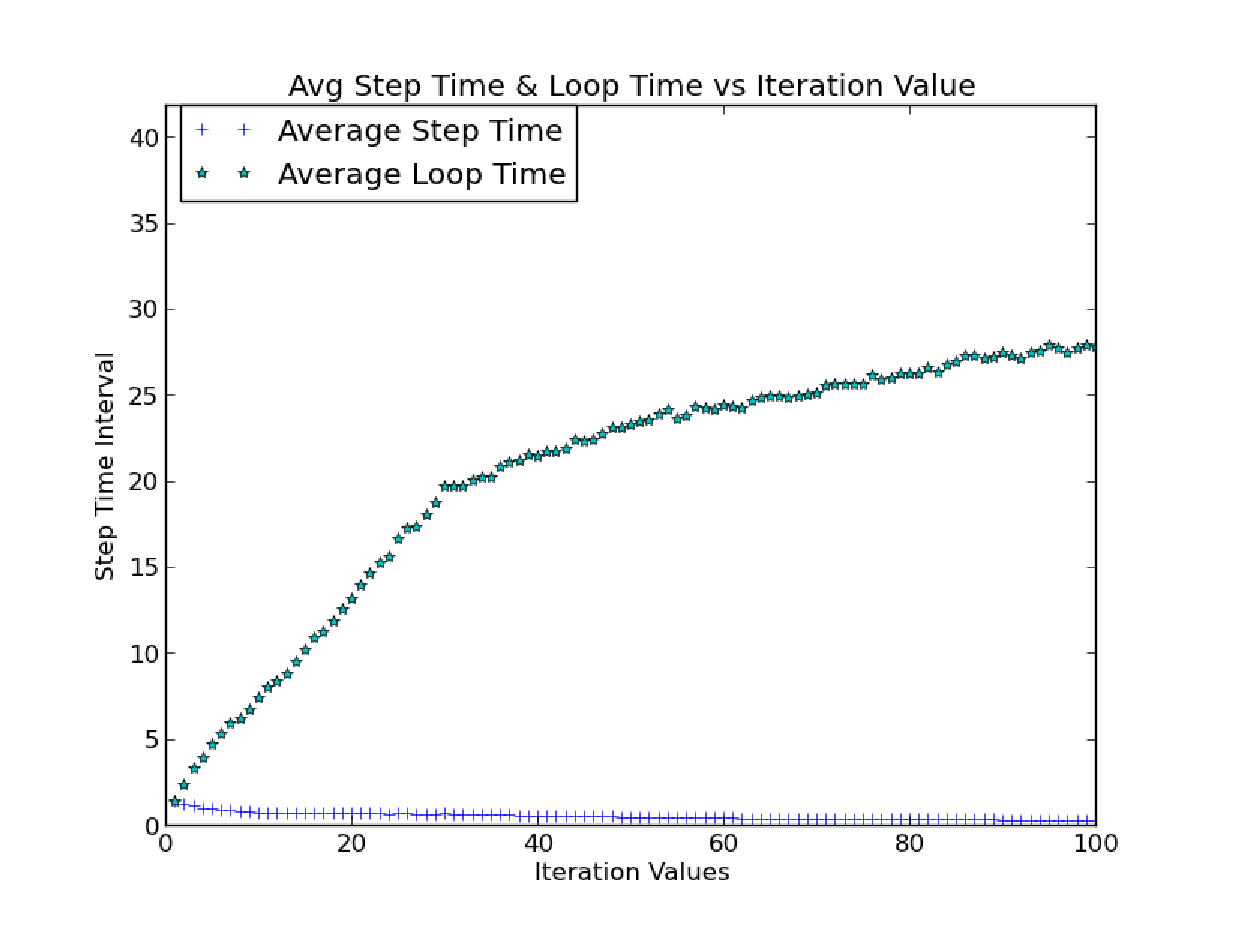
\includegraphics[width = 6cm]{plots-normal/l1.eps}
%\emph{Plot1 for normal \& heavy loaded system }
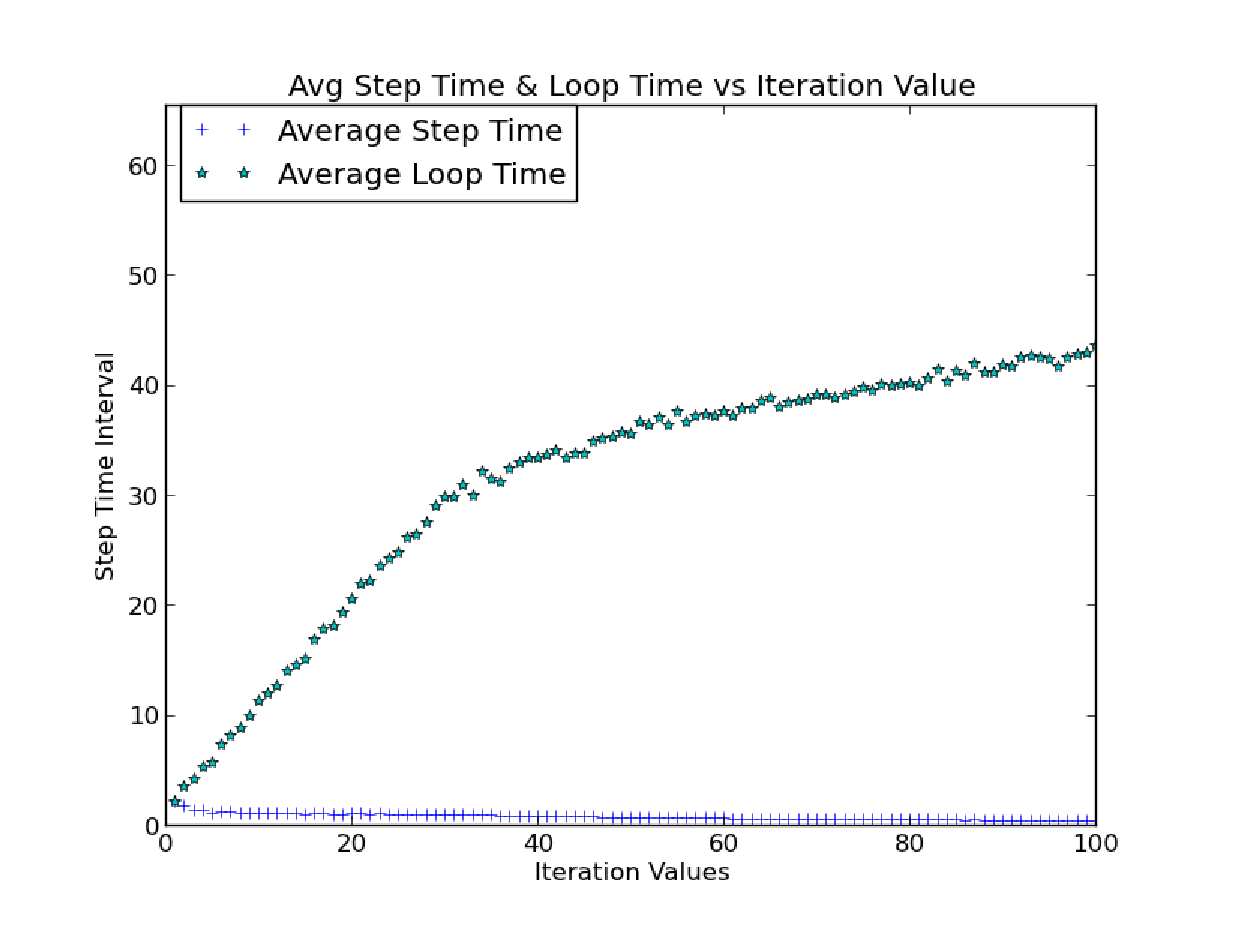
\includegraphics[width = 6cm]{plots-high/h1.eps}
\end{center}

This is a plot between the Average Step time and Average Loop Time (average with respect to the number of reruns) against the iteration number. \\
We observe that the avg step time per iteration slightly decreases as the number of iterations increase. This could be because computation for larger iterations are done efficiently using values from previous iterations.  The Avg loop time increases with the iterations. This is so because more time would be taken for more iterations. However the increase in loop time decreases with the iterations because of the decreasing trend of the step time. Ave Step time * Iterations turns out to be approximately equal to the loop time for all the runs. This shows the consistency between the b2Profile timers and the gettimeofday function. \\
The above was the case when system was normally loaded. When the system is heavily loaded, the nature of the plots is similar but they are shifted vertically upwards, as it takes more amount of time for the system to execute the same process. This is probably  because the slightly lower priority is given for scheduling of this process as compared to the the heavy ones. Also make plot02 target takes a lot more time to generate plots.
% This is measured by the time command on the command line.
   

\subsection{Average Collision Time , Velocity \& Position Updates Vs Iteration Values}

\begin{center}
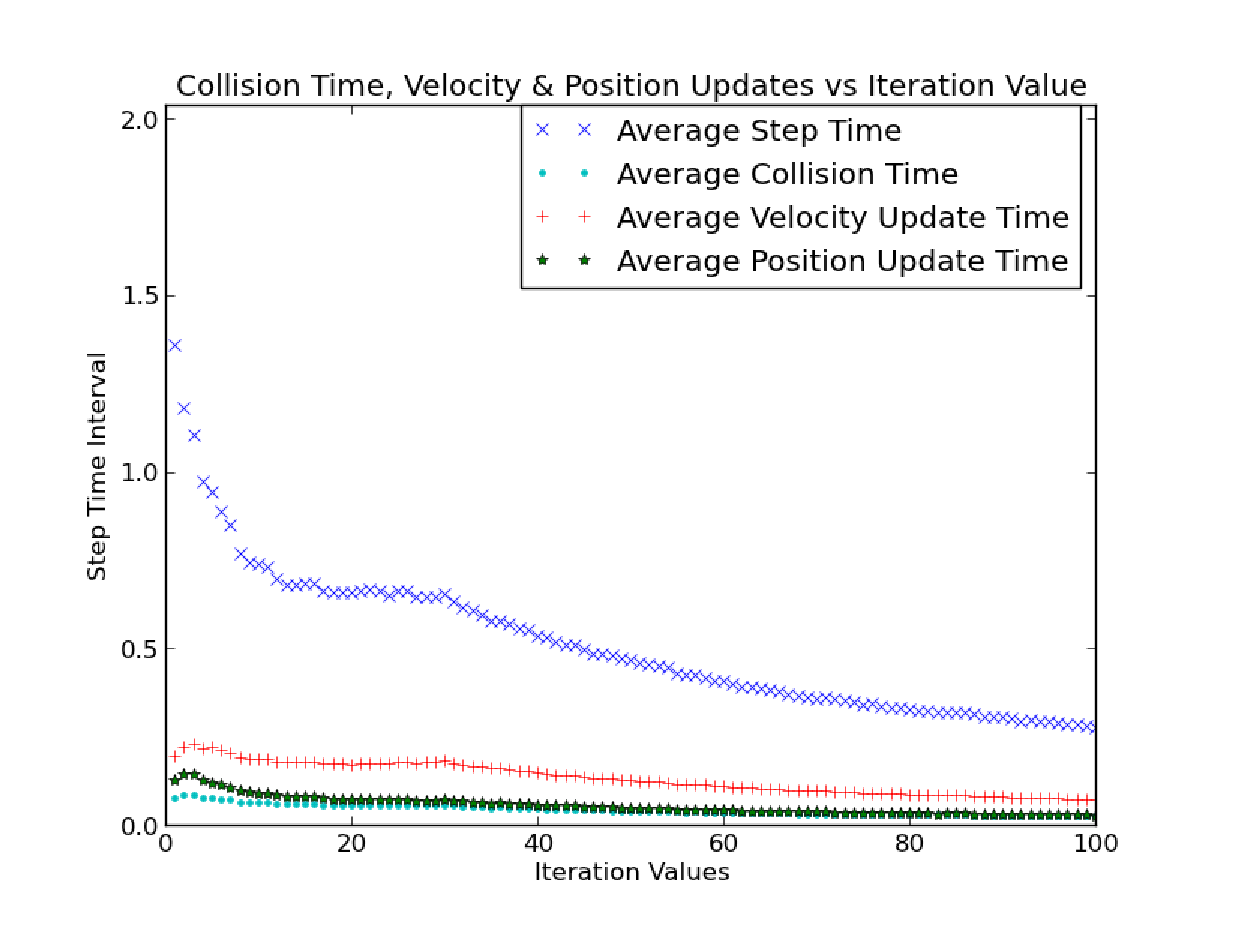
\includegraphics[width = 6cm]{plots-normal/l2.eps}
%\emph{Plot1 for normal \& heavy loaded system }
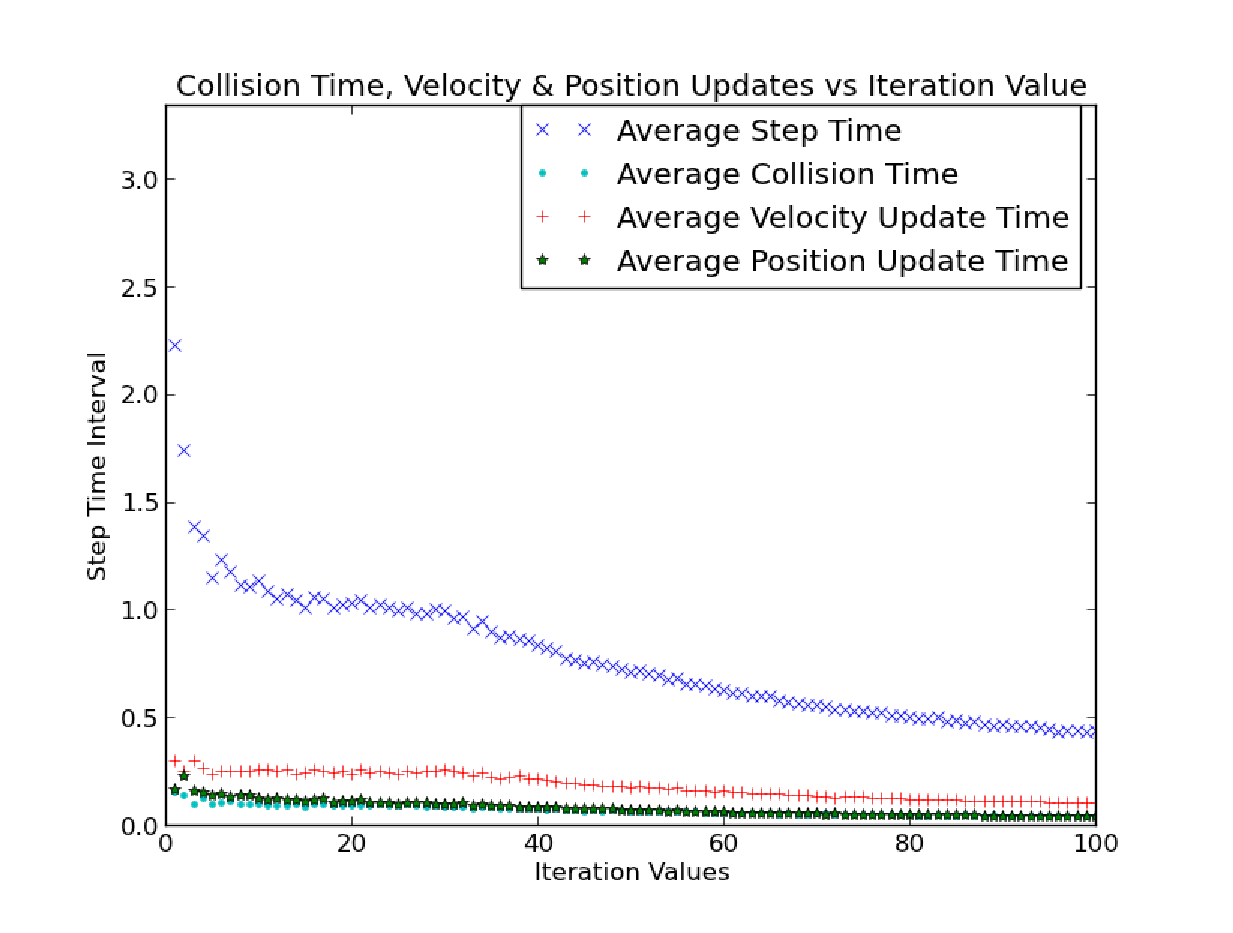
\includegraphics[width = 6cm]{plots-high/h2.eps}
\end{center}

The collision time , velocity updates , and position updates (all average with respect to reruns) also form a decreasing trend with respect to iterations. This is quite similar to the trend in avg step time. We observe that avg collision time, avg velocity \& position updates are all less that the avg step time, in fact even their sum is slightly less than step time. Thus we can infer that there are still other events apart from collision, velocity \& position updates that occur in each step. This analysis was for for the  normally loaded system. \\
Plotting the same, when the system is heavily loaded only results in a plot with a similar trend but upward shifted. The system takes more time for the same when heavily loaded.

\subsection{Average Step Time \& Average Loop Time Vs Rerun Values}
\begin{center}
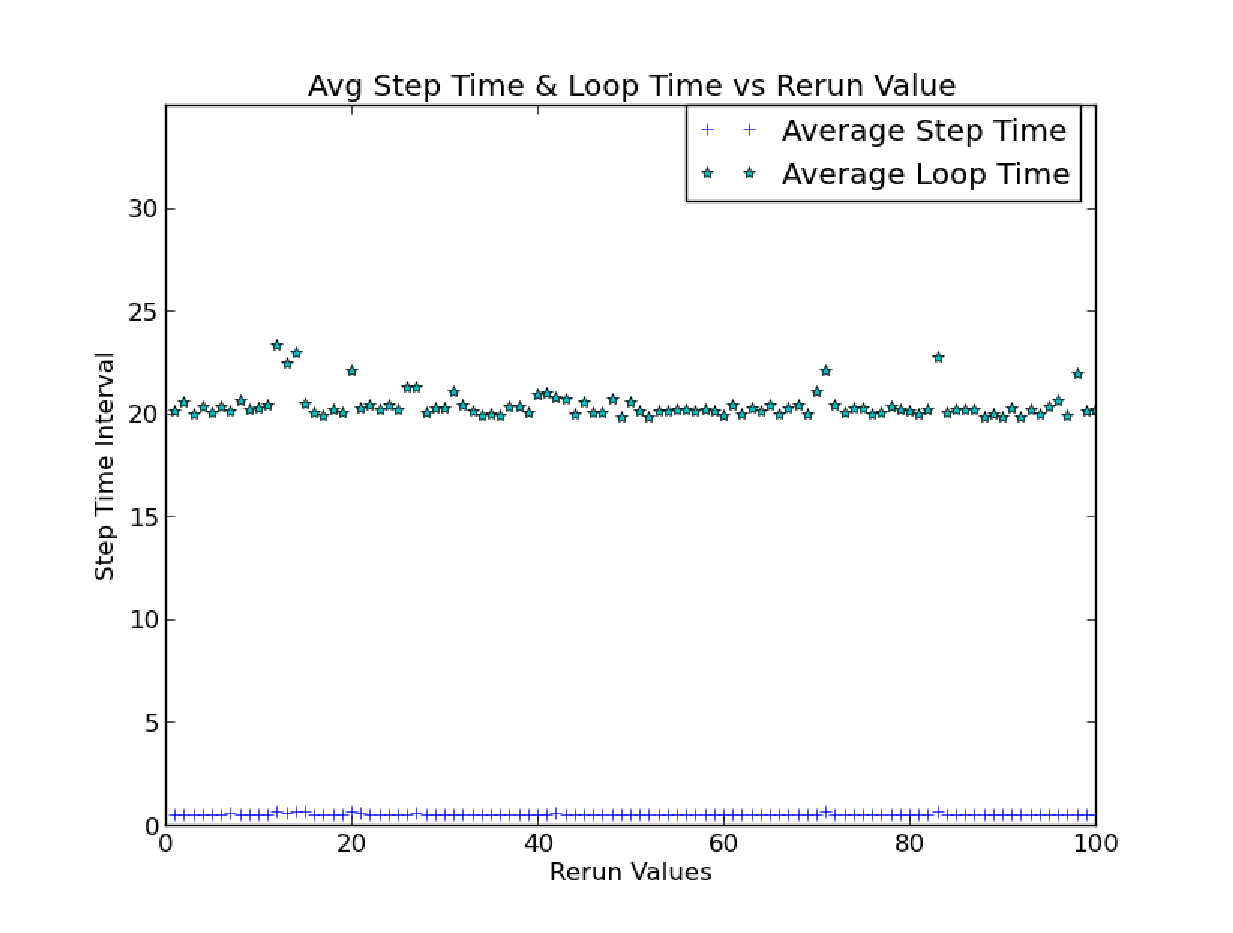
\includegraphics[width = 6cm]{plots-normal/l3.eps}
%\emph{Plot1 for normal \& heavy loaded system }
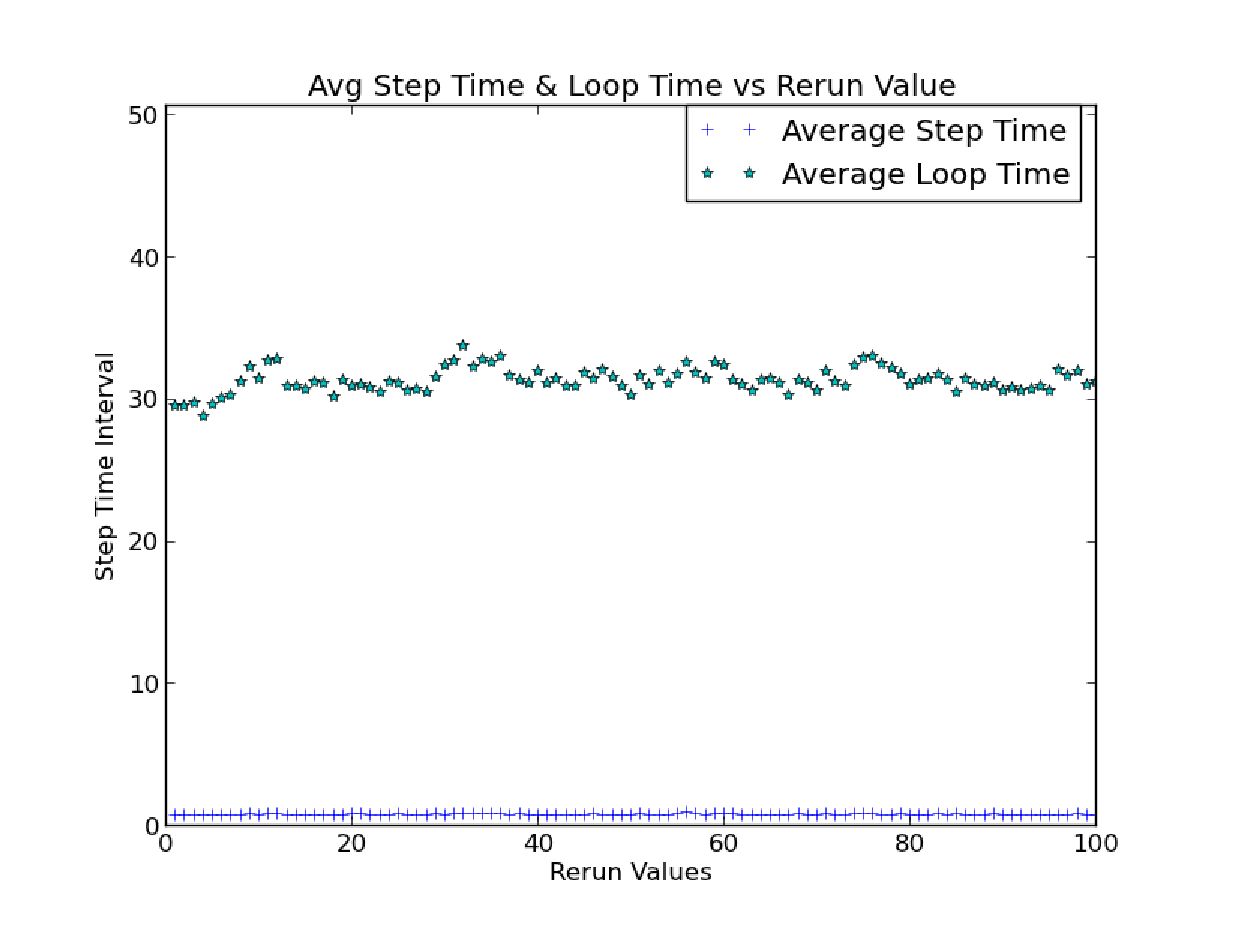
\includegraphics[width = 6cm]{plots-high/h3.eps}
\end{center}


The third plot is of Average Step time and Average Loop Time (average with respect to the number of iterations) against the rerun number. They show very less variation with reruns and are almost constant throughout. This shows the Step Time and Loop time don't depend on the number of reruns for any number of iterations and return almost the same value.\\
On plotting the above on a heavily loaded system , the same inference can be drawn. However the avg step time and avg loop time increases, due to high priority given to the heavy processes.

\subsection{Average Collision Time , Velocity \& Position Updates Vs Iteration Values}

\begin{center}
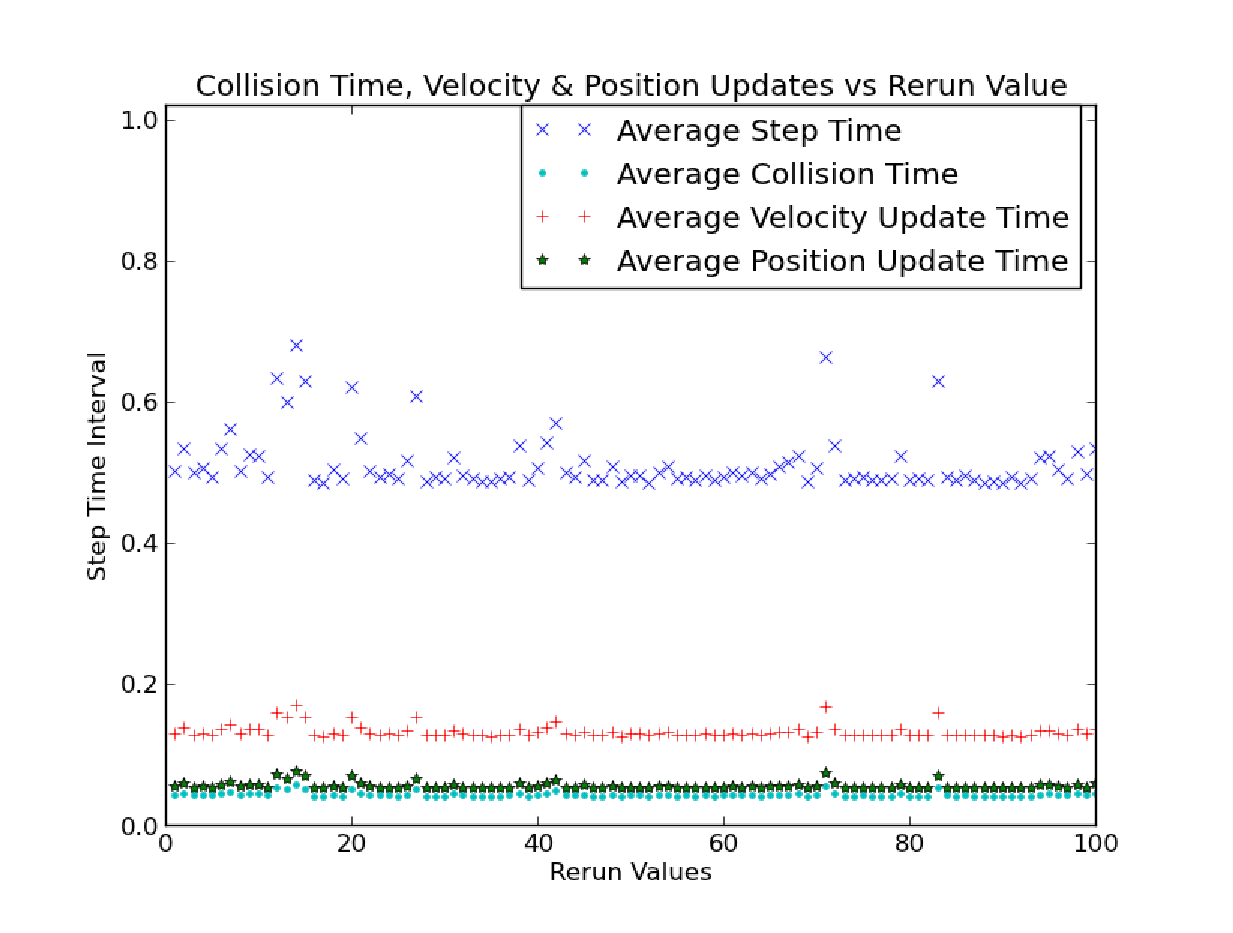
\includegraphics[width = 6cm]{plots-normal/l4.eps}
%\emph{Plot1 for normal \& heavy loaded system }
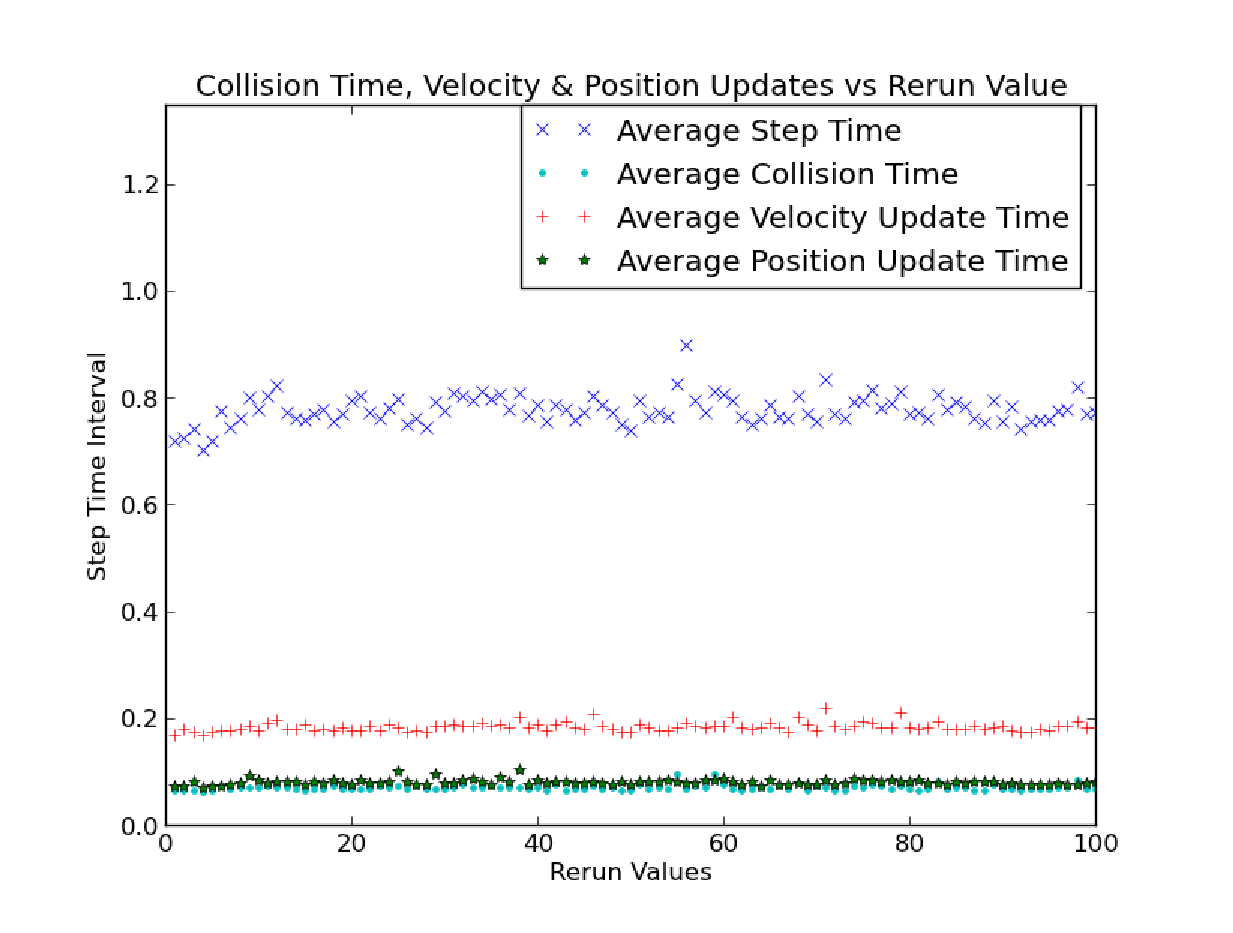
\includegraphics[width = 6cm]{plots-high/h4.eps}
\end{center}

This plot is of collision time , velocity updates , and position updates (all average with respect to the number of iterations) against the rerun number. The plot is nearly constant for all the three. Showing that there values don't change on running the code again. \\
On plotting with heavily loaded system, all the three increase but remain constant similar to the previous case.

\subsection{Step Time (with error-bars) Vs Iteration Values}
\begin{center}
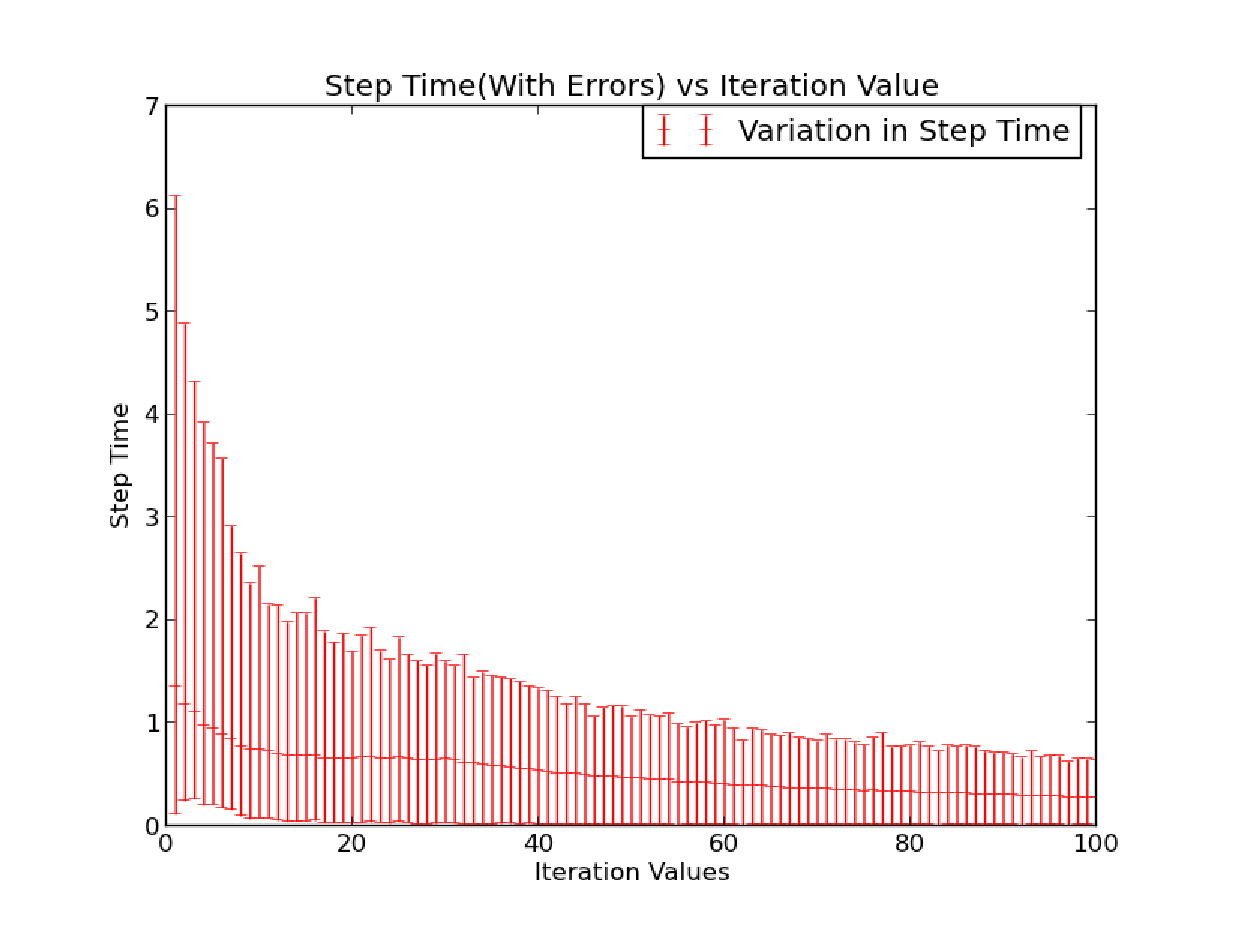
\includegraphics[width = 6cm]{plots-normal/l5.eps}
%\emph{Plot1 for normal \& heavy loaded system }
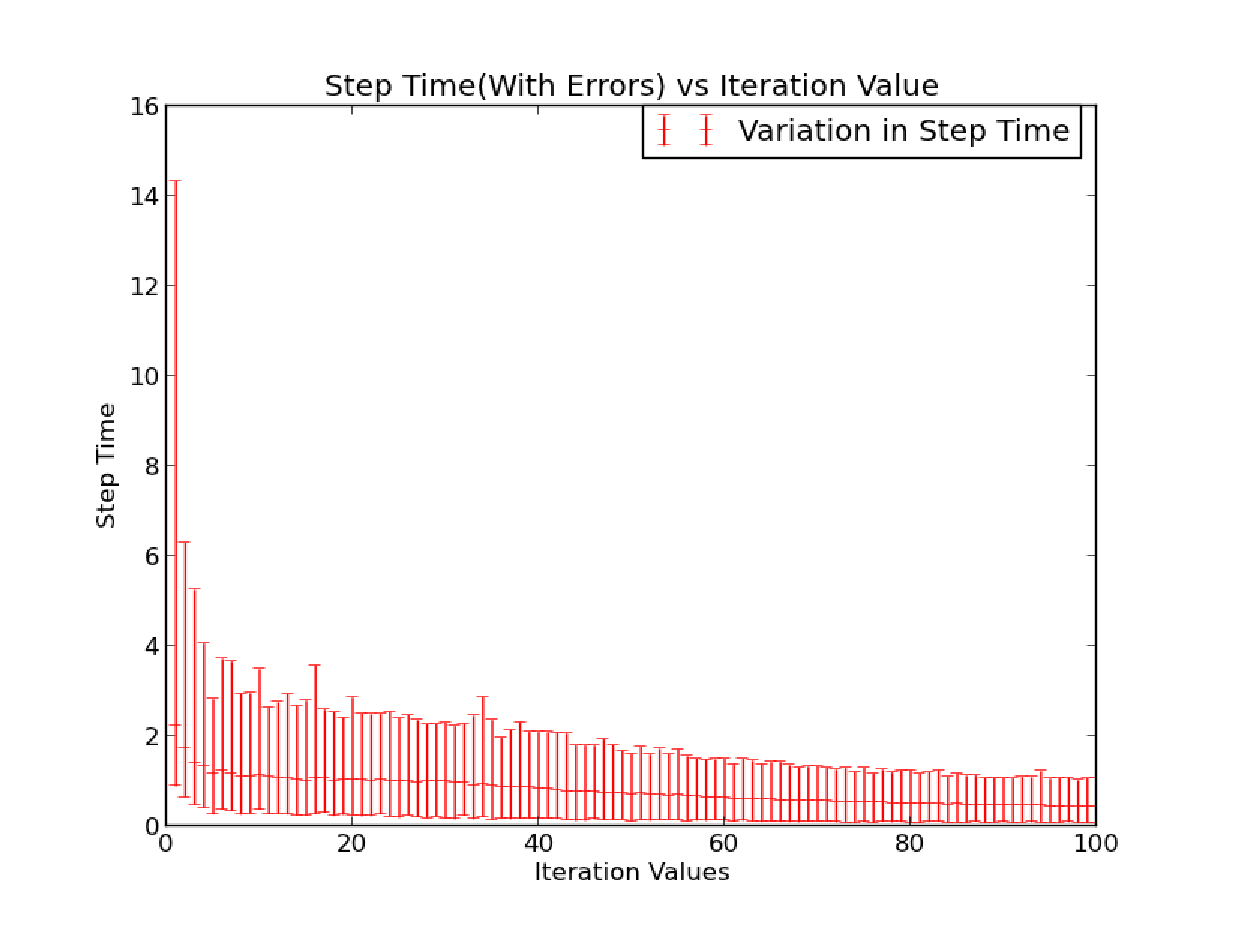
\includegraphics[width = 6cm]{plots-high/h5.eps}
\end{center}


This is a plot of avg step time (with error bars) with the iterations. The step time follows a decreasing trend with iterations, as observed earlier. From this plot, it is observed that the error in the avg step time decreases as the iterations progress. Relative error slightly decreases. Thus we get a good approximate for the average step time for larger number of iterations. Thus there should exist sufficient number of iterations in the computation to obtain the less variation in step time.\\
Only difference for a heavily loaded system,is that graph is only scaled and follows the same trend.

\subsection{Step Time frequency \& cumulative frequency plot (for a fixed iteration value)}

\begin{center}
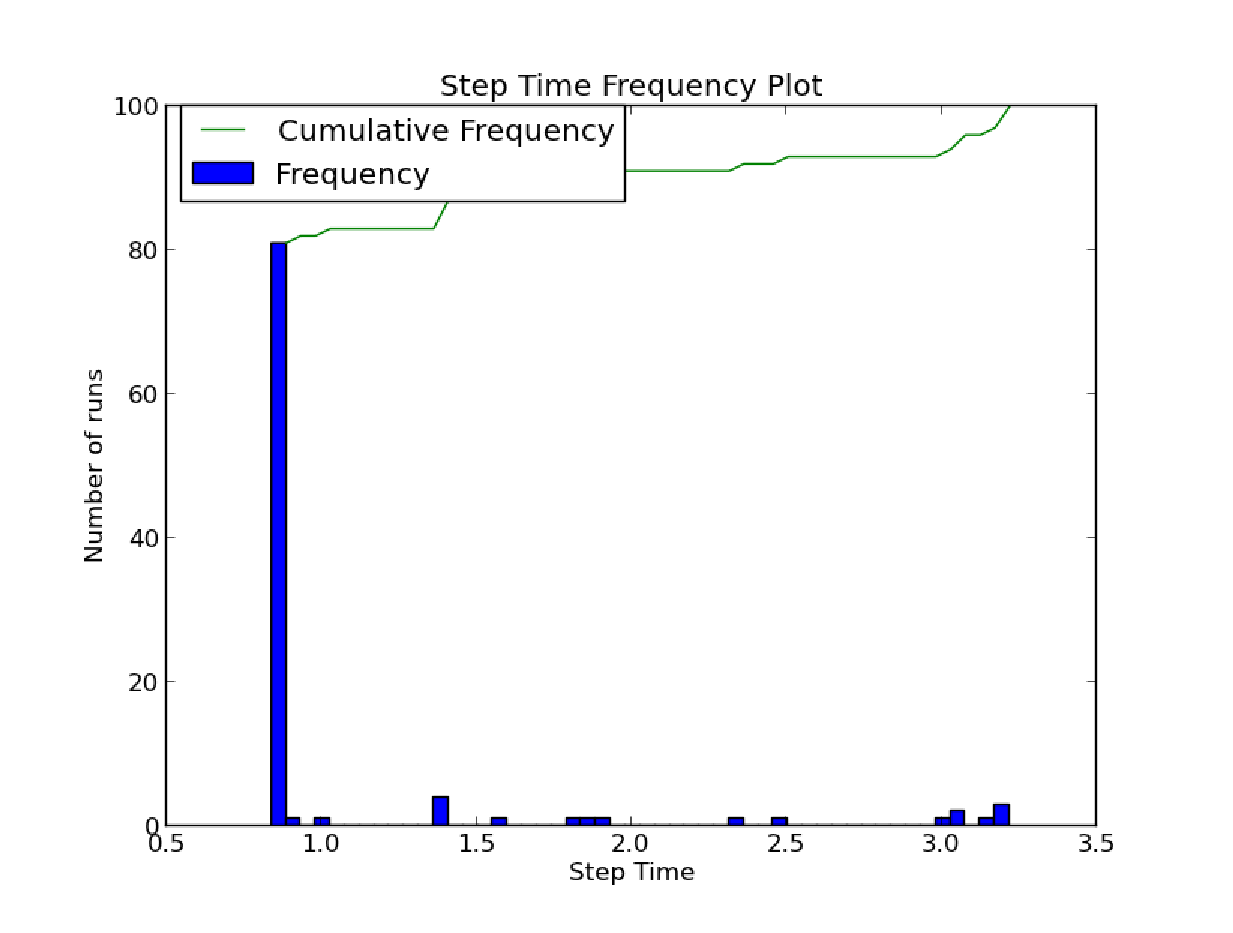
\includegraphics[width = 6cm]{plots-normal/l6.eps}
%\emph{Plot1 for normal \& heavy loaded system }
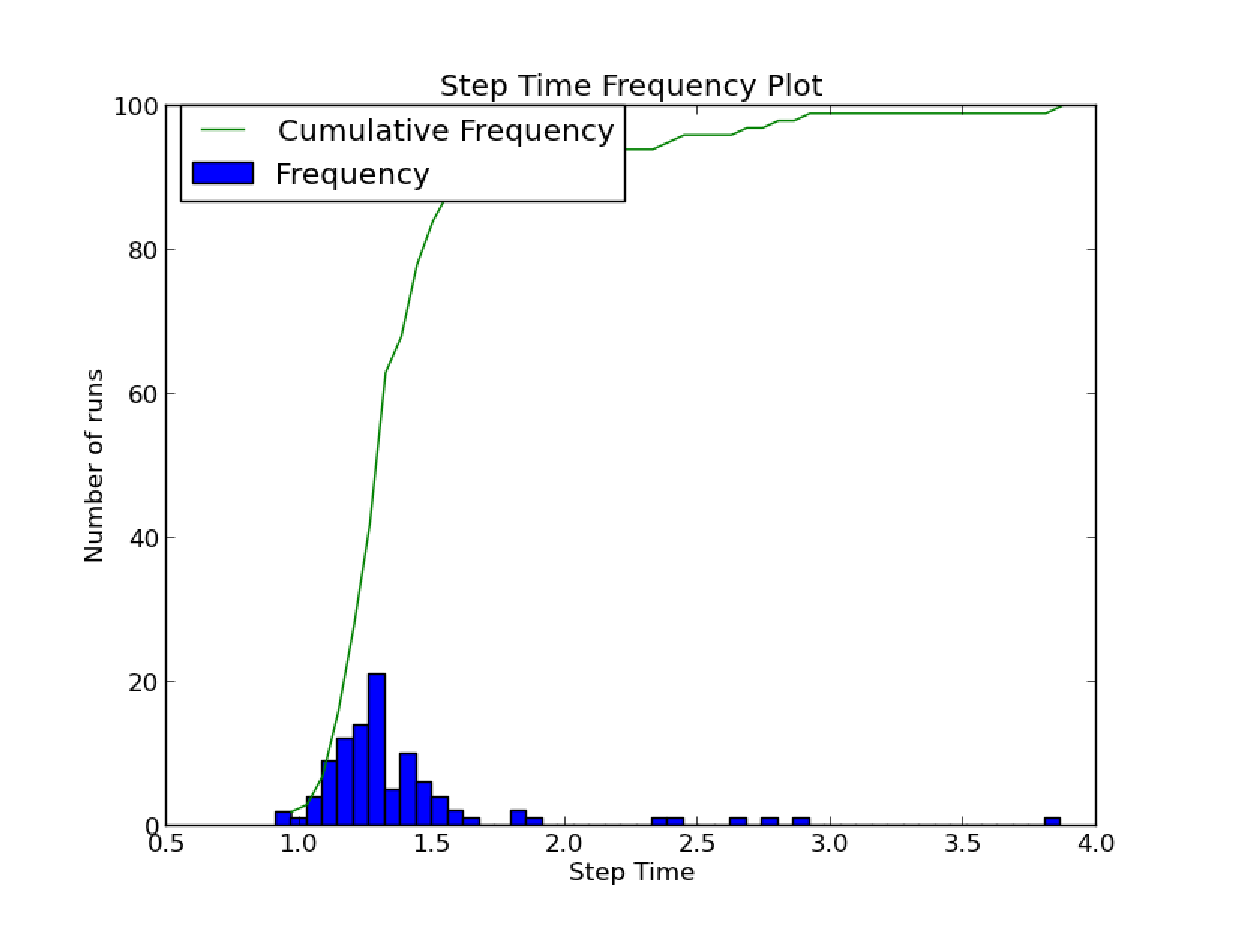
\includegraphics[width = 6cm]{plots-high/h6.eps}
\end{center}
This is a plot of frequency \& cumulative frequency distribution of step time (wrt no of reruns keeping iterations fixed). For the case of normally loaded system, the histogram has a random distribution(mostly uniform).There is not much difference between the number of	reruns for any intervals. The cumulative frequency distribution is plotted accordingly and is an increasing function.\\
For a heavily loaded system, the histogram is approximately follows the normal distribution. Maximum number of reruns occurs for an intermediate middle value. This is because of the resource constarints of processor and memory.




%%%%%%%%%%%%%%%%%%%%%%%ANMOL%%%%%%%%%%%%%%%%%%%%%%%%%%%%%%%%%%%%%%%%%%%%%%%%%%%%%%%%%%%
\section{Comparing the compiled code} 
This section draws inferences from the profiled data stored for different modes of compilation and compares them.
The code is compiled in \textbf{Release mode} using optimisation flags(-O2 or -O3) as compared to \textbf{Debug mode}. This way the GCC compiler will try to optimize the program and make it run faster but at the same time increase compile time and memory consumpttion. The following points can be inferred from the profiled data : 

\begin{itemize}
\item Total time taken in Debug mode : 8.87 secs
\item Total time taken in Release mode : 2.14 secs
\item Functions with the most number of calls : b2ContactSolver::SolveVelocityConstraints()
\end{itemize}

The following parts of the code seems to take a lot of time as concluded by the call graph. A breif explanantion of how GCC might have optimised the code is also given.
\begin{enumerate}
\item \textbf{b2ContactSolver::SolveVelocityConstraints()} : This is the most time consuming function which can be seen from the self time field in the call graph. 
\begin{itemize}
\item Time taken by this function call in debug mode = 1.65 secs
\item time taken by this function call in release mode = 0.96 secs
\end{itemize}
\begin{center}
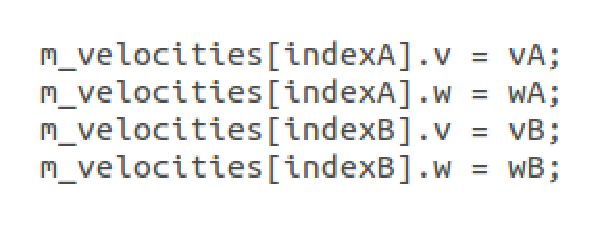
\includegraphics{ReportImages/point1.eps}
\end{center}
This is mainly because of the portion of the code described above in which we are doing redundant array indexing which is ultimately optimised in release mode.


\item \textbf{Optimization using -floop-optimizations} : b2Vec2::b2Vec2(float, float) is called the most number of times as can be seen from the number of calls field in call graph.
\begin{itemize}
\item Number of calls in Debug mode = 447140438 calls for 100000 iterations   
\item Number of calls in Release mode = 0 calls
\end{itemize}
\begin{center}
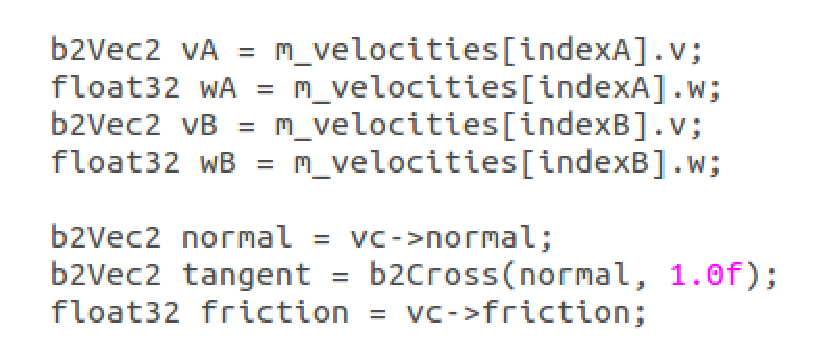
\includegraphics{ReportImages/point2.eps}
\end{center}
This is mainly because of the portion of the code described above in which we are declaring a b2Vec2(float, float) object inside the loop. This way we are allocating memory to the variables again and again for each iteration which is ultimately getting deallocated when the iteration ends. \\
Instead of this what we could have done is allocate memory to this object outside the loop which saves the time of reallocation of memory for each iteration value.

\item \textbf{Optimization using -finline-functions} : This is one of the many optimization techniques in which the call to the function is instead replaced by function defintion thus reducing the time in calling and returning the child function for each parent function. This can be seen clearly in the call graph for release and debug modes where the multilevel dense debug tree is just replaced by a single level release tree mainly because of inline function optimization. 


\end{enumerate}

\section{Analysis of the Call Graph}
A call graph is a directed graph that represents calling relationships between callee and caller functions in a computer program. Each node represents a function and a edge from function f to g indicates that procedure f calls procedure g. \\
Each node also includes the percentage of the total time that was spent in this function and its children. The percentage written in the angular bracket for each node denotes the percentage of the total time that was spent in this function.
Each edge label denotes the number of calls to the child function invoked by the node function.
 

\begin{center}
\includegraphics[scale=0.2]{ReportImages/debug_prof.eps} \\
\emph{Call graph for Debug mode}
\end{center}


As we can see the call graph for Debug is dense and includes many nodes and edges which is what we expected.

\begin{center}
\includegraphics[scale=0.3]{ReportImages/release_prof.eps} \\
\emph{Call graph for Release mode}
\end{center}



The call graph for Release is flat as it has been optimised, so all the redundant function calls and loops have been optimised.

\section{Optimizations in dominos.cpp}
The following are the optimizations which can be done in the dominos.cpp improve the performance of the code.

\begin{itemize}

\item Instead of defining new Fixture Definitions to the each and every body we can reuse the same varibale by reassigning it different values. Same goes for Body Definitions. This would improve the performance of the code and result in less calls to the constructor.
\item Another instance where the code can be optimized is in the system of pendulums and dominos. In this we have declared all the variables inside the body of the loop. They can be declared outside and reassigned at every iteration at every iteration.

\end{itemize}



\bibliographystyle{plain}
\bibliography{Ref}
\center{[Prepared in \LaTeX{} \cite{Wiki}]}

\end{document}








